\documentclass[12pt, letterpaper]{article}

\usepackage{graphicx}

\begin{document}
\setlength\parindent{0pt}
\textbf{
1.1.9\\
Given:
\[ y' + 4y = 1.4,\; y = ce^{-4x} + 0.35,\; y(0) = 2 \]
(a) Verify that $y$ is a solution of the ODE.\\
(b) Determine from $y$ the particular solution of the IVP.\\
(c) Graph the solution of the IVP.
}

\vspace{5mm}
\textit{Solution to (a):}\\
We can verify that $y$ is a solution of the ODE by differntiating y 
and plugging $y$ and $y'$ into the ODE. Given:
\[ y = ce^{-4x} + 0.35 \]
Then:
\[ y' = -4ce^{-4x} \]
And, plugging $y$ and $y'$ into our ODE:
\[ -4ce^{-4x} + 4(ce^{-4x} + 0.35) = 1.4 \]
Simplifying:
\[ -4ce^{-4x} + 4ce^{-4x} + 4*0.35 = 1.4 \]
Finally:
\[ 1.4 = 1.4 \]
Proving that $y = ce^{-4x} + 0.35$ is a valid solution to the ODE.

\vspace{5mm}
\textit{Solution to (b):}
Given: $y(0) = 2$ and $y = ce^{-4x} + 0.35$, we can solve for $c$:
\[ 2 = ce^{-4(0)} + 0.35 \]
Then:
\[ c = \frac{2-0.35}{e^0} = 1.65 \]
Thus, the particular solution is:
\[ y = 1.65e^{-4x} + 0.35\]

\newpage
\textit{Solution to (c):}
The plot of the particular solution is shown in Figure 1.

\begin{figure}
\centering
  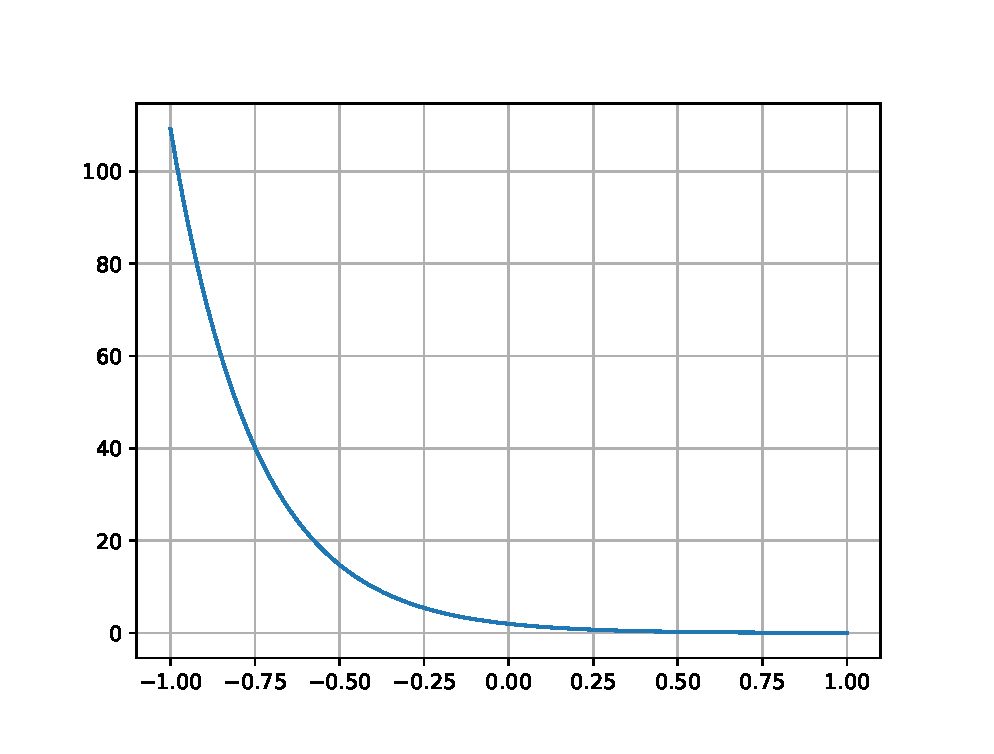
\includegraphics[width=0.8\textwidth]{1.1.9_graph.eps}
\caption{graph of the particular solution to 1.1.9.}
\label{fig:1.1.9}
\end{figure}

\end{document}